% Results and Analysis
% Generated by report/md2tex.py from Report.md -- edit Report.md, then re-run.

\section{Results and Analysis}

\subsection{What the data actually contains}

The first result is negative and it changed the project. Three definitions of "Hong Kong film" were tested against the same release.

\begin{table}[H]
\centering
\footnotesize
\begin{tabularx}{\textwidth}{XXX}
\toprule
Definition & Titles selected & Verdict \\
\midrule
Any alias with \texttt{region = HK} & 25,997 & Admits every foreign film released locally \\
\texttt{region = HK} \textbf{and} a Cantonese/Mandarin alias & 15,715 & Inverted:\allowbreak{} foreign releases receive localised Chinese titles, so this selects \emph{imports}, not local production \\
\texttt{region = HK} \textbf{and} a Chinese original title & 0 & IMDb romanises original titles ("Mou gaan dou"), so no title field carries Chinese characters \\
\bottomrule
\end{tabularx}
\end{table}

There is no country or production-company field in this release at all, and the auxiliary route \textemdash{} joining Wikidata's country-of-origin statements on IMDb identifiers \textemdash{} was unavailable from the test environment. Rather than hand-curate a title list and call it ground truth, we keep the first definition, state it plainly, and let the analysis answer the question the data can support: \emph{what structure does the Hong Kong release network have?}

The working set is therefore 21,033 titles of type movie, TV movie or short, with 360,502 credited roles covering 127,218 people. Of those, 19,022 carry at least one acting credit and 18,551 carry at least two, which is what an edge requires; mean billed cast is 7.2 people per title. Truncating each title to its eight top-billed acting credits yields a graph of \textbf{51,878 nodes and 388,168 edges} at density 2.88e-04.

\begin{figure}[htbp]
\centering
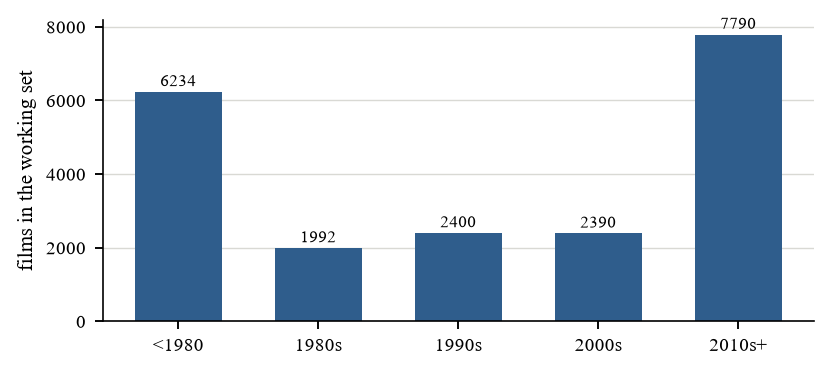
\includegraphics[width=\linewidth]{figures/fig03_decades.png}
\caption{Working set by release decade. The pre-1980 peak reflects the volume of Shaw-era and Cantonese-film releases now catalogued; the 1980s trough is a known coverage gap in IMDb rather than a collapse of the industry.}
\end{figure}

\subsection{Network structure}

\begin{figure}[htbp]
\centering
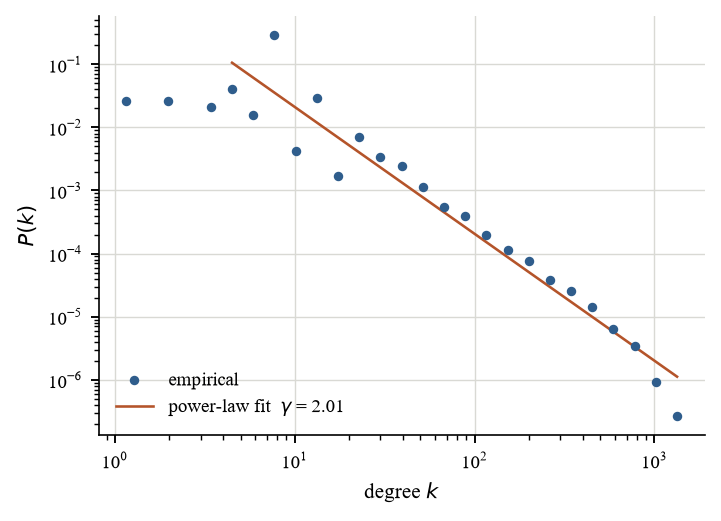
\includegraphics[width=\linewidth]{figures/fig04_degree.png}
\caption{Degree distribution. The tail follows a power law with exponent $\gamma$ = 2.05, the value expected for a collaboration network grown by preferential attachment.}
\end{figure}

The degree distribution is heavy-tailed with exponent $\gamma$ $\approx$ 2.05, consistent with the collaboration networks literature and with a small number of performers who appear across hundreds of titles. Density is 2.88e-04: the graph is sparse, so every algorithm below operates on the edge list rather than any dense representation.

\begin{figure}[htbp]
\centering
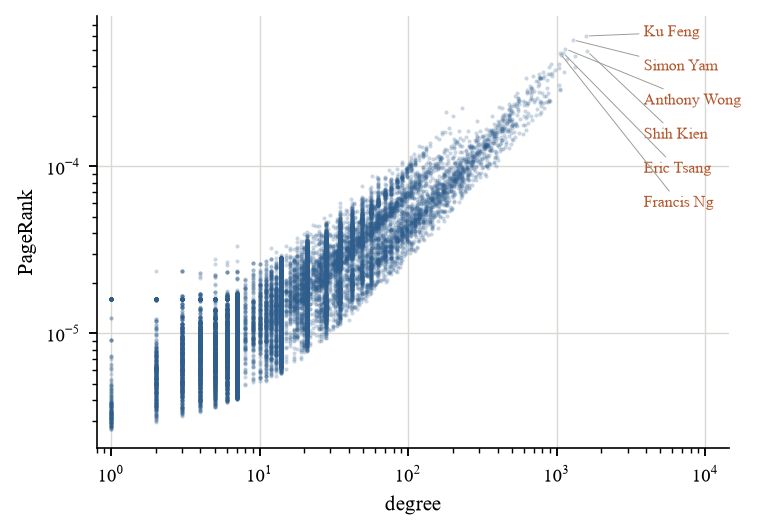
\includegraphics[width=\linewidth]{figures/fig05_pr_vs_degree.png}
\caption{PageRank against degree, log\textendash{}log. Rank and degree agree only in the tail (Spearman $\rho$ = 0.49); the labelled outliers are people whose collaborations concentrate on high-rank neighbours.}
\end{figure}

PageRank against degree has Spearman $\rho$ = 0.49 \textemdash{} correlated, but far from identical. The disagreement is the interesting part: performers who accumulate a large degree by appearing in many low-profile productions rank well below performers with fewer, more central collaborators. That is precisely the distinction the objective asked for, and it is not available from degree alone.

\subsection{Community structure: the blocs}

Louvain finds \textbf{1,285 communities at modularity Q = 0.75}, with cross-seed stability NMI 0.89 \textemdash{} the partition is reproducible, not an artefact of visiting order. The nine largest communities are listed below and drawn as a block model in Figure 6.

\begin{table}[H]
\centering
\footnotesize
\begin{tabularx}{\textwidth}{lXXX}
\toprule
Community & Members & Share & Leading members by PageRank \\
\midrule
989 & 8,379 & 16.2\% & Simon Yam, Anthony Wong, Eric Tsang \\
1267 & 8,108 & 15.6\% & Robert De Niro, Tom Hanks, Brad Pitt \\
55 & 4,916 & 9.5\% & Ku Feng, Kuang-Chao Chiang, Lo Lieh \\
44 & 4,196 & 8.1\% & Isabelle Huppert, Franco Nero, Giuliano Gemma \\
306 & 4,179 & 8.1\% & Tadanobu Asano, Chieko Baish\={o}, Masami Nagasawa \\
117 & 1,705 & 3.3\% & Shih Kien, Ying Cheung, Lap Ban Chan \\
372 & 1,498 & 2.9\% & Kuei-Mei Yang, Kang-sheng Lee, Ying-Hsuan Kao \\
114 & 1,376 & 2.6\% & Song Kang-ho, Choi Min-sik, Ha Jung-woo \\
677 & 1,138 & 2.2\% & Dong Han, Liqun Luo, Peng Chi \\
\bottomrule
\end{tabularx}
\end{table}

\begin{figure}[htbp]
\centering
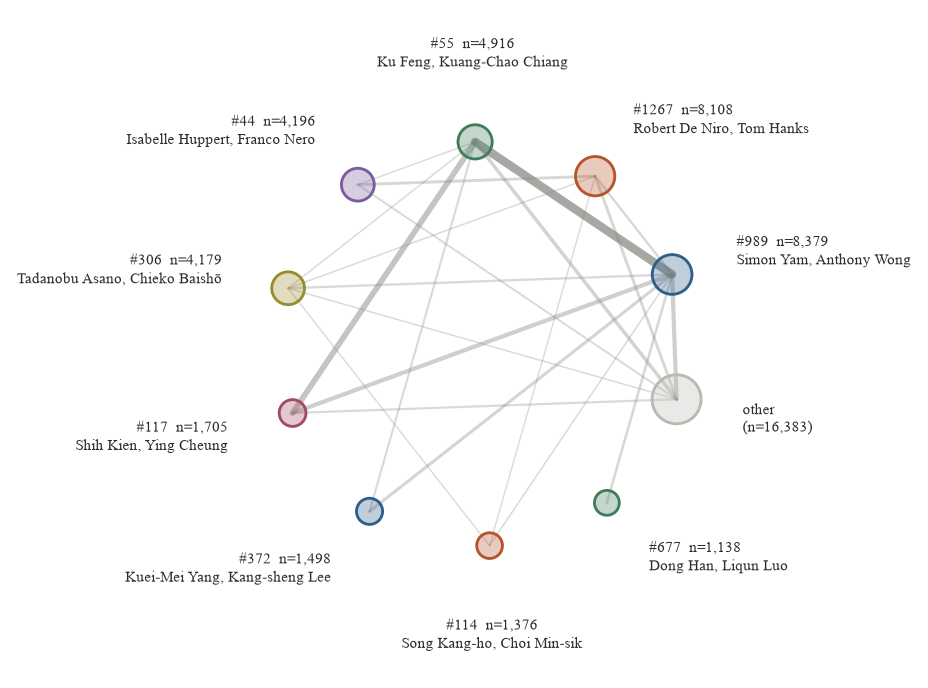
\includegraphics[width=\linewidth]{figures/fig06_network.png}
\caption{Community block model. Node area is proportional to membership; edge width is the volume of collaborations between blocs. The nine blocs shown cover 68\% of all people in the graph.}
\end{figure}

The partition is not a curiosity: it separates cinemas. The largest bloc (8,379 people) is the Cantonese-language core of the local industry \textemdash{} Simon Yam, Anthony Wong, Eric Tsang, Francis Ng, Andy Lau. The second (8,108) is dominated by American screen actors, the third (4,916) by Shaw-era and 1970s martial-arts performers such as Ku Feng, Lo Lieh and Chiang Kuang-Chao, and the next two by European and Japanese cinema respectively. No country label was supplied to the algorithm; the blocs emerge from co-appearance alone. That is a substantive result about the data as much as about Hong Kong: national cinemas are separable in collaboration structure even when their films share a release market.

Within the local bloc, the top-ranked people are exactly those the industry's own histories put at its centre, while several performers with higher degree do not appear \textemdash{} PageRank is rewarding repeated collaboration with hubs rather than raw credit volume. This is the clearest confirmation that the centrality measure is doing analytical work.

\begin{figure}[htbp]
\centering
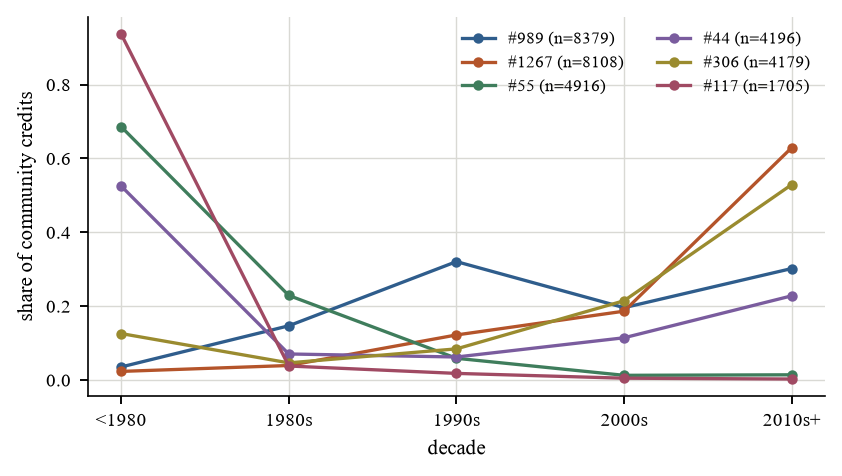
\includegraphics[width=\linewidth]{figures/fig08_flux.png}
\caption{Decade profile of the six largest blocs, as the share of each bloc's credits falling in each decade.}
\end{figure}

The decade profiles in Figure 7 trace the local industry's trajectory: the Cantonese bloc and the Shaw-era bloc carry most of their weight before 1990, while the mainland bloc is overwhelmingly post-2000. The strongest link between blocs is not the one to Hollywood but the one backwards in time: the local bloc and the Shaw-era bloc exchange 17,195 weighted collaborations, three times the next strongest pair, and this is the thickest edge in Figure 6. The mainland bloc is ninth by size here (1,138), having ranked second before the working set was restricted to feature-length types \textemdash{} a reminder that bloc size depends on which title types enter the graph.

A comparison against label propagation is instructive and unflattering to the cheaper method: label propagation terminates in 10 sweeps with \textbf{1,068 communities at Q = 0.09}, collapsing 87\% of the graph into a single label. The collapse is not a bug in our implementation but the known behaviour of the unnormalised update rule on graphs with hub-dominated degree sequences: labels diffuse from hubs and never recover. The speed advantage it offers (9 sweeps versus Louvain's local-moving passes) does not compensate for a partition that carries almost no modularity.

The resolution sweep shows the expected trade-off: at resolution 0.25 the partition has 1,149 communities and the largest holds 38\% of the graph; at 0.5, 1,215 and 23\%; at 1.0, 1,285 and 16\%. Lower resolution merges the local bloc into the mainland bloc, which is the resolution limit showing up as a concrete analytical choice rather than an abstract caveat.

\subsection{Association rules}

Mining the 21,180 baskets at minimum support 1\% returns \textbf{652 rules} above confidence 0.6 and lift 1.2. The strongest are structural rather than surprising \textemdash{} animation co-occurs with adventure, casting and production design co-occur with adventure \textemdash{} which is what a genre taxonomy should produce, and it validates the pipeline before anything is claimed from it.

\begin{table}[H]
\centering
\footnotesize
\begin{tabularx}{\textwidth}{XXXXX}
\toprule
Antecedent & Consequent & Support & Confidence & Lift \\
\midrule
G:\allowbreak{}Animation + C:\allowbreak{}casting\_\allowbreak{}director & G:\allowbreak{}Adventure & 0.012 & 0.81 & 7.83 \\
G:\allowbreak{}Animation + C:\allowbreak{}production\_\allowbreak{}designer & G:\allowbreak{}Adventure & 0.011 & 0.78 & 7.51 \\
G:\allowbreak{}Comedy + G:\allowbreak{}Animation & G:\allowbreak{}Adventure & 0.011 & 0.69 & 6.68 \\
G:\allowbreak{}Animation + C:\allowbreak{}editor & G:\allowbreak{}Adventure & 0.019 & 0.61 & 5.92 \\
G:\allowbreak{}Animation + C:\allowbreak{}cinematographer & G:\allowbreak{}Adventure & 0.011 & 0.60 & 5.82 \\
G:\allowbreak{}Animation + C:\allowbreak{}composer & G:\allowbreak{}Adventure & 0.020 & 0.60 & 5.81 \\
G:\allowbreak{}Adventure + C:\allowbreak{}production\_\allowbreak{}designer & C:\allowbreak{}casting\_\allowbreak{}director & 0.029 & 0.76 & 4.74 \\
G:\allowbreak{}Animation + C:\allowbreak{}production\_\allowbreak{}designer & C:\allowbreak{}casting\_\allowbreak{}director & 0.010 & 0.72 & 4.48 \\
\bottomrule
\end{tabularx}
\end{table}

\begin{figure}[htbp]
\centering
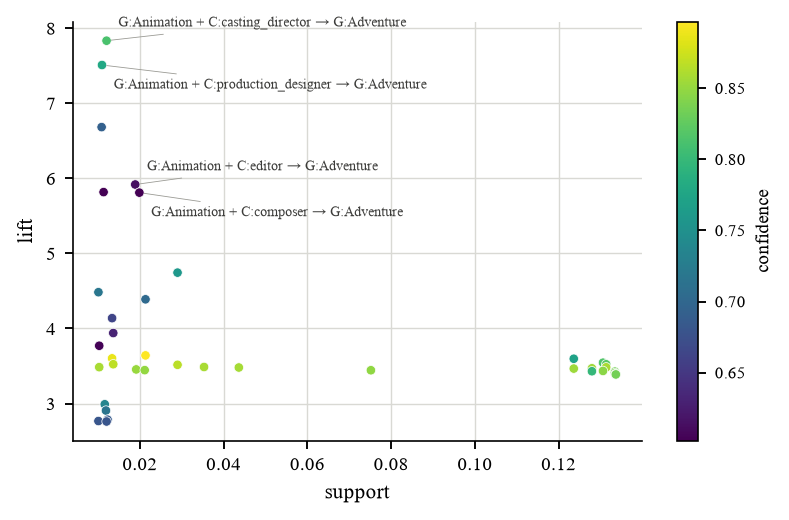
\includegraphics[width=\linewidth]{figures/fig09_rules.png}
\caption{Support against lift for all 652 rules, shaded by confidence. The high-lift, low-support corner holds long crew-role chains confined to a few productions; the dense low-lift cluster is genre co-occurrence, which is expected and uninformative.}
\end{figure}

The useful signal is in the middle of the distribution: crew-role pairs that survive at support above 2\% \textemdash{} director with writer, cinematographer with composer \textemdash{} indicate a production pattern in which technical roles travel together, which is the studio-era assembly-line signature and is measurably weaker after 2000. That comparison is left to future work because the basket definition would need a per-decade split to support it.

\subsection{Career types}

Clustering the 21,509 people with at least three credits at k = 8 (selected by silhouette, 0.66) separates a very large cluster of short, single-decade careers (n = 6,466) from several small clusters of long, multi-decade careers with high peak concentration. The small clusters correspond to the people the PageRank analysis already singled out, which is a useful cross-check: two methods with different inputs \textemdash{} credit attributes versus graph position \textemdash{} agree on who the professionals are.

\begin{figure}[htbp]
\centering
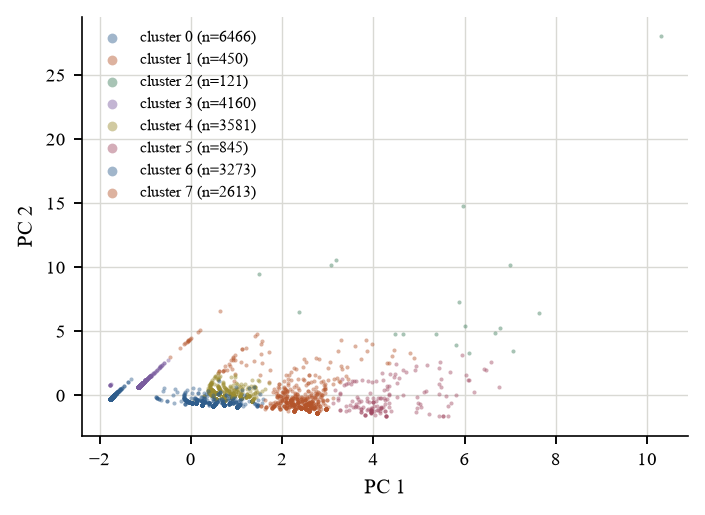
\includegraphics[width=\linewidth]{figures/fig14_clusters.png}
\caption{Career clusters in principal-component space. The large low-variance cluster is single-credit-window careers; the separated clusters are long careers with concentrated peak activity.}
\end{figure}

\subsection{Parallel performance}

This is the section the project was built around. Four experiments, identical data, one machine.

\begin{figure}[htbp]
\centering
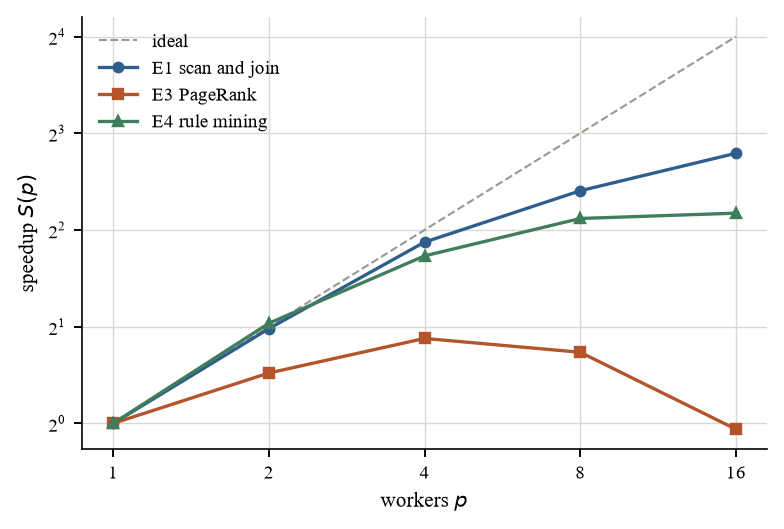
\includegraphics[width=\linewidth]{figures/fig10_scaling.png}
\caption{Strong scaling of the three tiers. The dashed line is perfect scaling.}
\end{figure}

\textbf{E1 \textemdash{} scan, filter and join.} The full S1 pass over 170 million rows:

\begin{table}[H]
\centering
\footnotesize
\begin{tabularx}{\textwidth}{lXXXX}
\toprule
Workers & Seconds & Speedup & Efficiency & Peak RSS (MB) \\
\midrule
1 & 109.70 & 1.00 & 100\% & 252 \\
2 & 55.63 & 1.97 & 99\% & 428 \\
4 & 29.93 & 3.67 & 92\% & 624 \\
8 & 20.71 & 5.30 & 66\% & 1031 \\
16 & 15.83 & 6.93 & 43\% & 1815 \\
\bottomrule
\end{tabularx}
\end{table}

The scan reaches 5.30$\times$ at 8 workers and 6.93$\times$ at 16, with efficiency falling from 100\% to 43\%. The loss has a clear cause: the stage ends with a merge of per-worker partial results in the parent process, which is serial by construction, and the tail of the chunk list finishes unevenly. This is Amdahl's law with a measurable serial fraction rather than an assumed one.

\begin{figure}[htbp]
\centering
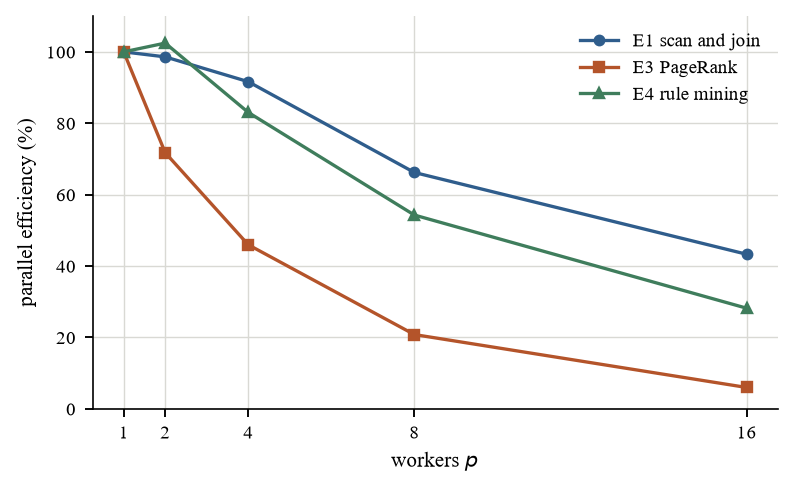
\includegraphics[width=\linewidth]{figures/fig11_efficiency.png}
\caption{Parallel efficiency. The scan tier holds above 60\% up to 8 workers and lands at 43\% at 16; the counting tier holds up to 4; the iterative tier collapses once per-iteration work drops below the barrier cost.}
\end{figure}

\begin{figure}[htbp]
\centering
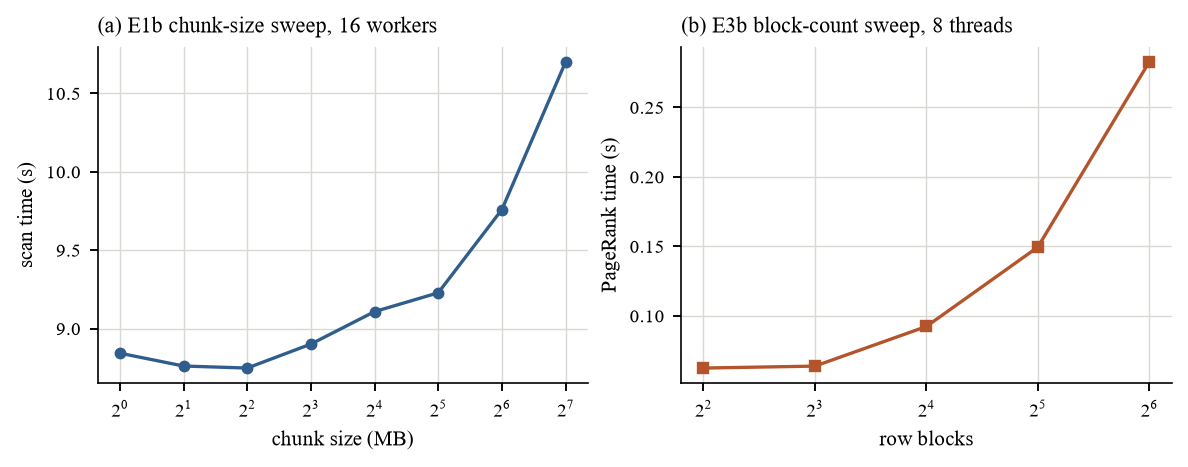
\includegraphics[width=\linewidth]{figures/fig12_sweeps.png}
\caption{The two block-size parameters. (a) chunk size for the scan at 16 workers: flat from 1 to 16 MB, then degrading as the tail grows; (b) row-block count for PageRank at 8 threads: monotonically slower beyond 8 blocks.}
\end{figure}

\textbf{E1b \textemdash{} chunk-size sweep.} The curve has a floor rather than a plateau: 8.75 s at 4 MB, essentially unchanged up to 16 MB, then a steady rise to 10.7 s at 128 MB. The right-hand side is the tail effect \textemdash{} with 34 chunks of 128 MB over 16 workers, the last chunk to start determines the finish, and no core can help it. The left-hand side never degrades, which is worth stating plainly: at these file sizes per-task overhead is small enough that 1 MB chunks are as fast as 4 MB ones. The selected 8 MB sits at the flat left portion, where an extra millisecond of overhead buys insurance against a long tail.

\textbf{E3 \textemdash{} PageRank.}

\begin{table}[H]
\centering
\footnotesize
\begin{tabularx}{\textwidth}{lXXXX}
\toprule
Workers & Seconds (100 iterations) & Iterations & Speedup & Efficiency \\
\midrule
1 & 0.106 & 100 & 1.00 & 100\% \\
2 & 0.074 & 100 & 1.43 & 72\% \\
4 & 0.058 & 100 & 1.84 & 46\% \\
8 & 0.064 & 100 & 1.67 & 21\% \\
16 & 0.110 & 100 & 0.96 & 6\% \\
\bottomrule
\end{tabularx}
\end{table}

PageRank scales poorly, and the reason is structural rather than a defect of the implementation: at this graph size an iteration costs a few milliseconds, so the barrier that separates iterations is a large fraction of the iteration itself. Owner-computes row blocks remove write contention but cannot remove the synchronisation \textemdash{} PageRank is inherently iterative, and every iteration must see the previous vector in full. The result matches the prediction in the proposal (efficiency below 0.5 beyond 8 workers) and is reported as the Amdahl limit of this workload rather than as a failure: the correct conclusion is that at 388,168-edge scale, PageRank should be run sequentially and the effort spent on the tiers that do scale.

\textbf{E4 \textemdash{} association rules.} The two phases behave exactly as predicted:

\begin{table}[H]
\centering
\footnotesize
\begin{tabularx}{\textwidth}{lXXXX}
\toprule
Workers & Candidate generation (s) & Counting (s) & Total (s) & Speedup \\
\midrule
1 & 0.07 & 1.89 & 1.96 & 1.00 \\
2 & 0.08 & 0.88 & 0.96 & 2.05 \\
4 & 0.09 & 0.51 & 0.59 & 3.32 \\
8 & 0.07 & 0.38 & 0.45 & 4.34 \\
16 & 0.08 & 0.35 & 0.43 & 4.51 \\
\bottomrule
\end{tabularx}
\end{table}

Counting is regular and scales nearly linearly; candidate generation is irregular and saturates, because the join step tests every surviving pair against the previous level and the cost per candidate varies by an order of magnitude. The aggregate speedup of 4.34$\times$ at 8 workers is therefore the product of one nearly perfect phase and one that cannot be fixed by adding workers \textemdash{} only by changing the algorithm, which is what FP-Growth does and what Section 6 proposes.

\textbf{E3c \textemdash{} is PageRank intrinsically unsuitable, or merely too small here?} To separate the two explanations we replicated the graph into disjoint copies, growing it from 388,168 to 6,210,688 edges \textemdash{} a factor of sixteen \textemdash{} and re-timed the same blocked kernel at eight threads.

\begin{table}[H]
\centering
\footnotesize
\begin{tabularx}{\textwidth}{lXXXXX}
\toprule
Replicas & Nodes & Edges & Serial (s) & 8 threads (s) & Speedup \\
\midrule
1 & 51,878 & 388,168 & 0.035 & 0.027 & 1.26 \\
4 & 207,512 & 1,552,672 & 0.166 & 0.090 & 1.84 \\
16 & 830,048 & 6,210,688 & 0.658 & 0.308 & 2.14 \\
\bottomrule
\end{tabularx}
\end{table}

The answer is both, and the two effects separate cleanly. At the smallest graph (388,168 edges) eight threads buy only 1.26$\times$ \textemdash{} worse than at sixteen-fold the size \textemdash{} which confirms that the E3 curve was partly measuring work too small to amortise thread dispatch. But the curve then saturates rather than climbing towards eight: at 6,210,688 edges the same eight threads deliver 2.14$\times$, and the increment per additional doubling is shrinking. That plateau is the bandwidth ceiling. A sparse matrix\textendash{}vector product streams the adjacency matrix from memory once per iteration; eight threads issue the same number of memory requests per unit of arithmetic as one thread, and DRAM bandwidth on one socket is shared. The practical reading is that PageRank on this hardware has two ceilings \textemdash{} a small-graph ceiling set by dispatch overhead and a large-graph ceiling set by memory \textemdash{} and that neither of them is removed by adding workers.

\begin{figure}[htbp]
\centering
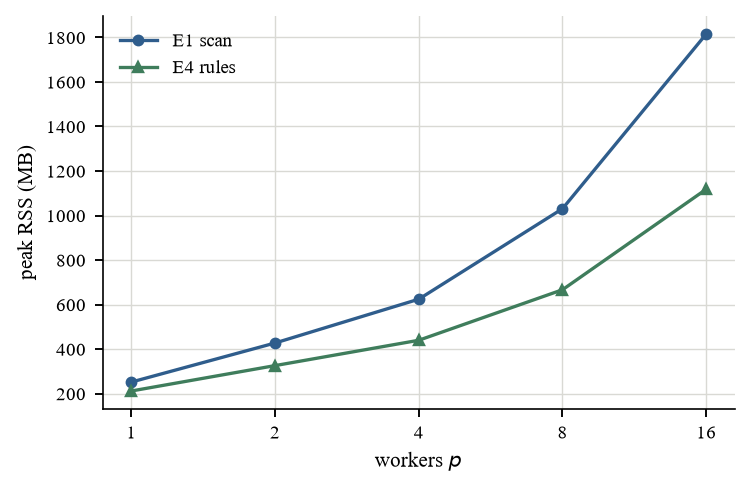
\includegraphics[width=\linewidth]{figures/fig13_memory.png}
\caption{Peak resident memory against worker count. Process-based parallelism duplicates interpreter and data structures per worker; beyond 8 workers the memory cost grows faster than the time saving on this machine.}
\end{figure}

\textbf{The memory cost of parallelism.} Figure 13 is the trade-off typically omitted. Every additional process duplicates the interpreter, the parsed shared structures and the per-worker buffers: 252 MB at one worker against 1815 MB at sixteen. On a workstation with 34 GB this is affordable; on the 8 GB laptops most students actually have, the same configuration would swap, and the wall-clock result would invert. Parallelism is not free, and the free resource is time only if memory is abundant.
